\documentclass[aspectratio=169,10pt]{beamer}
\usetheme{Madrid}
\usecolortheme{whale}
\usepackage{pgfplots}
\pgfplotsset{compat=1.18}
\usepackage{booktabs}
\usepackage{amsmath}

\pgfplotsset{
  every axis/.style={
    width=6.5cm, height=5cm,
    grid=major, grid style={dashed,gray!40},
    mark size=1.5pt,
    xlabel={$p$},
    xmin=0, xmax=1.0,
    xticklabel style={/pgf/number format/fixed, /pgf/number format/precision=2},
  },
  black line/.style={
    smooth, thick, black,
  },
}

\title{Capacity with Haircut vs.\ Capacity=Supply (p=0..1)}
\subtitle{exp_min_p_0_1\_capacity\_haircut vs.\ exp_min_p_0_1\_capacity\_supply}
\author{}
\date{\today}

\begin{document}

\begin{frame}
  \titlepage
\end{frame}

\begin{frame}{Bankruptcies (exp_min_p_0_1\_capacity\_haircut)}
  \begin{columns}[T]
    \begin{column}{0.55\textwidth}
      \begin{figure}
        \centering
        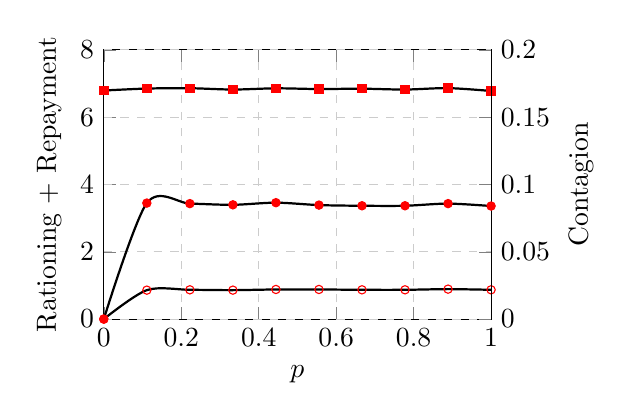
\begin{tikzpicture}
        \begin{axis}[
          ylabel={Rationing + Repayment},
          ymin=0, ymax=8,
          xmin=0, xmax=1.0,
          xticklabel style={/pgf/number format/fixed, /pgf/number format/precision=2},
        ]
          \addplot[only marks, mark=square*, red] coordinates {
            (0.00001,6.7930)            (0.11112,6.8513)            (0.22223,6.8612)            (0.33334,6.8222)            (0.44445,6.8584)            (0.55556,6.8366)            (0.66667,6.8472)            (0.77778,6.8218)            (0.88889,6.8642)            (1.00000,6.7793)
          };
          \addplot[black line] coordinates {
            (0.00001,6.7930)            (0.11112,6.8513)            (0.22223,6.8612)            (0.33334,6.8222)            (0.44445,6.8584)            (0.55556,6.8366)            (0.66667,6.8472)            (0.77778,6.8218)            (0.88889,6.8642)            (1.00000,6.7793)
          };
          \addplot[only marks, mark=o, red] coordinates {
            (0.00001,0.00)            (0.11112,0.86)            (0.22223,0.87)            (0.33334,0.86)            (0.44445,0.88)            (0.55556,0.88)            (0.66667,0.87)            (0.77778,0.87)            (0.88889,0.89)            (1.00000,0.87)
          };
          \addplot[black line] coordinates {
            (0.00001,0.00)            (0.11112,0.86)            (0.22223,0.87)            (0.33334,0.86)            (0.44445,0.88)            (0.55556,0.88)            (0.66667,0.87)            (0.77778,0.87)            (0.88889,0.89)            (1.00000,0.87)
          };
        \end{axis}
        \begin{axis}[
          ylabel={Contagion},
          ymin=0, ymax=0.2,
          xmin=0, xmax=1.0,
          axis y line*=right, axis x line=none,
          ylabel near ticks,
          yticklabel style={/pgf/number format/fixed, /pgf/number format/precision=2},
        ]
          \addplot[only marks, mark=*, red] coordinates {
            (0.00001,0.0000)            (0.11112,0.0862)            (0.22223,0.0858)            (0.33334,0.0849)            (0.44445,0.0865)            (0.55556,0.0847)            (0.66667,0.0842)            (0.77778,0.0842)            (0.88889,0.0858)            (1.00000,0.0840)
          };
          \addplot[black line] coordinates {
            (0.00001,0.0000)            (0.11112,0.0862)            (0.22223,0.0858)            (0.33334,0.0849)            (0.44445,0.0865)            (0.55556,0.0847)            (0.66667,0.0842)            (0.77778,0.0842)            (0.88889,0.0858)            (1.00000,0.0840)
          };
        \end{axis}
        \end{tikzpicture}
      \end{figure}
    \end{column}
    \begin{column}{0.42\textwidth}
      \tiny
      Bankruptcies:
      \begin{enumerate}
        \item[] $\blacksquare$ \textbf{Rationing.}
        \item[] $\bullet$ \textbf{Contagion.}
        \item[] $\circ$ \textbf{Failed repayment.}
      \end{enumerate}
      \tiny\renewcommand{\arraystretch}{0.85}\setlength{\tabcolsep}{2pt}
      \begin{tabular}{lccc}
        \toprule
        $p$ & Rat. & Cont. & Fail. \\
        \midrule
        0.00001 & 6.79 & 0.00 & 0.00 \\
        0.111 & 6.85 & 0.09 & 0.86 \\
        0.222 & 6.86 & 0.09 & 0.87 \\
        0.333 & 6.82 & 0.08 & 0.86 \\
        0.444 & 6.86 & 0.09 & 0.88 \\
        \textbf{0.556} & \textbf{6.84} & \textbf{0.08} & \textbf{0.88} \\
        0.667 & 6.85 & 0.08 & 0.87 \\
        0.778 & 6.82 & 0.08 & 0.87 \\
        0.889 & 6.86 & 0.09 & 0.89 \\
        1.000 & 6.78 & 0.08 & 0.87 \\
        \bottomrule
      \end{tabular}
    \end{column}
  \end{columns}
\end{frame}

\begin{frame}{Bankruptcies (exp_min_p_0_1\_capacity\_supply)}
  \begin{columns}[T]
    \begin{column}{0.55\textwidth}
      \begin{figure}
        \centering
        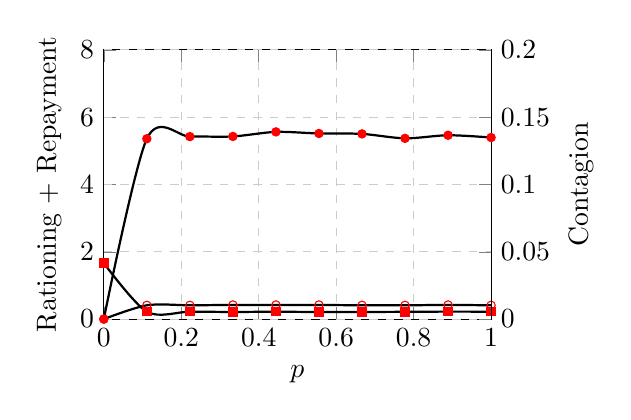
\begin{tikzpicture}
        \begin{axis}[
          ylabel={Rationing + Repayment},
          ymin=0, ymax=8,
          xmin=0, xmax=1.0,
          xticklabel style={/pgf/number format/fixed, /pgf/number format/precision=2},
        ]
          \addplot[only marks, mark=square*, red] coordinates {
            (0.00001,1.6644)            (0.11112,0.2170)            (0.22223,0.2205)            (0.33334,0.2114)            (0.44445,0.2184)            (0.55556,0.2100)            (0.66667,0.2110)            (0.77778,0.2160)            (0.88889,0.2219)            (1.00000,0.2194)
          };
          \addplot[black line] coordinates {
            (0.00001,1.6644)            (0.11112,0.2170)            (0.22223,0.2205)            (0.33334,0.2114)            (0.44445,0.2184)            (0.55556,0.2100)            (0.66667,0.2110)            (0.77778,0.2160)            (0.88889,0.2219)            (1.00000,0.2194)
          };
          \addplot[only marks, mark=o, red] coordinates {
            (0.00001,0.00)            (0.11112,0.41)            (0.22223,0.41)            (0.33334,0.42)            (0.44445,0.42)            (0.55556,0.42)            (0.66667,0.41)            (0.77778,0.41)            (0.88889,0.42)            (1.00000,0.41)
          };
          \addplot[black line] coordinates {
            (0.00001,0.00)            (0.11112,0.41)            (0.22223,0.41)            (0.33334,0.42)            (0.44445,0.42)            (0.55556,0.42)            (0.66667,0.41)            (0.77778,0.41)            (0.88889,0.42)            (1.00000,0.41)
          };
        \end{axis}
        \begin{axis}[
          ylabel={Contagion},
          ymin=0, ymax=0.2,
          xmin=0, xmax=1.0,
          axis y line*=right, axis x line=none,
          ylabel near ticks,
          yticklabel style={/pgf/number format/fixed, /pgf/number format/precision=2},
        ]
          \addplot[only marks, mark=*, red] coordinates {
            (0.00001,0.0000)            (0.11112,0.1340)            (0.22223,0.1356)            (0.33334,0.1357)            (0.44445,0.1391)            (0.55556,0.1379)            (0.66667,0.1376)            (0.77778,0.1343)            (0.88889,0.1366)            (1.00000,0.1349)
          };
          \addplot[black line] coordinates {
            (0.00001,0.0000)            (0.11112,0.1340)            (0.22223,0.1356)            (0.33334,0.1357)            (0.44445,0.1391)            (0.55556,0.1379)            (0.66667,0.1376)            (0.77778,0.1343)            (0.88889,0.1366)            (1.00000,0.1349)
          };
        \end{axis}
        \end{tikzpicture}
      \end{figure}
    \end{column}
    \begin{column}{0.42\textwidth}
      \tiny
      Bankruptcies:
      \begin{enumerate}
        \item[] $\blacksquare$ \textbf{Rationing.}
        \item[] $\bullet$ \textbf{Contagion.}
        \item[] $\circ$ \textbf{Failed repayment.}
      \end{enumerate}
      \tiny\renewcommand{\arraystretch}{0.85}\setlength{\tabcolsep}{2pt}
      \begin{tabular}{lccc}
        \toprule
        $p$ & Rat. & Cont. & Fail. \\
        \midrule
        0.00001 & 1.66 & 0.00 & 0.00 \\
        0.111 & 0.22 & 0.13 & 0.41 \\
        0.222 & 0.22 & 0.14 & 0.41 \\
        0.333 & 0.21 & 0.14 & 0.42 \\
        0.444 & 0.22 & 0.14 & 0.42 \\
        \textbf{0.556} & \textbf{0.21} & \textbf{0.14} & \textbf{0.42} \\
        0.667 & 0.21 & 0.14 & 0.41 \\
        0.778 & 0.22 & 0.13 & 0.41 \\
        0.889 & 0.22 & 0.14 & 0.42 \\
        1.000 & 0.22 & 0.13 & 0.41 \\
        \bottomrule
      \end{tabular}
    \end{column}
  \end{columns}
\end{frame}

\begin{frame}{Num. Loans: haircut ($\blacksquare$) vs.\ supply ($\circ$)}
  \begin{columns}[T]
    \begin{column}{0.55\textwidth}
      \begin{figure}
        \centering
        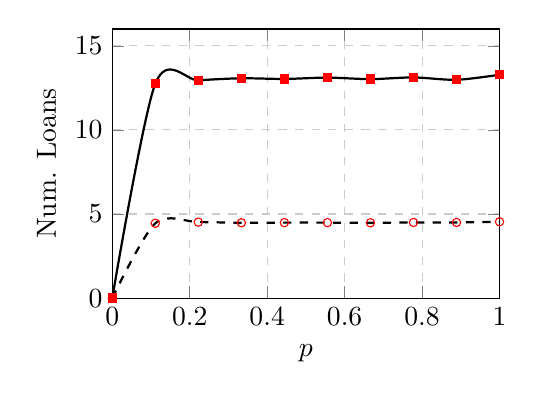
\begin{tikzpicture}
          \begin{axis}[
            ylabel={Num. Loans},
            ymin=0, ymax=16,
          ]
            \addplot[only marks, mark=square*, red] coordinates {
              (0.00001,0.00)            (0.11112,12.75)            (0.22223,12.95)            (0.33334,13.07)            (0.44445,13.03)            (0.55556,13.11)            (0.66667,13.02)            (0.77778,13.12)            (0.88889,12.98)            (1.00000,13.28)
            };
            \addplot[black line] coordinates {
              (0.00001,0.00)            (0.11112,12.75)            (0.22223,12.95)            (0.33334,13.07)            (0.44445,13.03)            (0.55556,13.11)            (0.66667,13.02)            (0.77778,13.12)            (0.88889,12.98)            (1.00000,13.28)
            };
            \addplot[only marks, mark=o, red] coordinates {
              (0.00001,0.00)            (0.11112,4.45)            (0.22223,4.52)            (0.33334,4.48)            (0.44445,4.49)            (0.55556,4.49)            (0.66667,4.48)            (0.77778,4.50)            (0.88889,4.50)            (1.00000,4.54)
            };
            \addplot[black line, dashed] coordinates {
              (0.00001,0.00)            (0.11112,4.45)            (0.22223,4.52)            (0.33334,4.48)            (0.44445,4.49)            (0.55556,4.49)            (0.66667,4.48)            (0.77778,4.50)            (0.88889,4.50)            (1.00000,4.54)
            };
          \end{axis}
        \end{tikzpicture}
      \end{figure}
    \end{column}
    \begin{column}{0.42\textwidth}
      \tiny\renewcommand{\arraystretch}{0.85}\setlength{\tabcolsep}{2pt}
      \begin{tabular}{lrr}
        \toprule
        $p$ & haircut & supply \\
        \midrule
        0.00001 & 0.00 & 0.00 \\
        0.111 & 12.75 & 4.45 \\
        0.222 & 12.95 & 4.52 \\
        0.333 & 13.07 & 4.48 \\
        0.444 & 13.03 & 4.49 \\
        \textbf{0.556} & \textbf{13.11} & \textbf{4.49} \\
        0.667 & 13.02 & 4.48 \\
        0.778 & 13.12 & 4.50 \\
        0.889 & 12.98 & 4.50 \\
        1.000 & 13.28 & 4.54 \\
        \bottomrule
      \end{tabular}
    \end{column}
  \end{columns}
\end{frame}

\begin{frame}{Leverage: haircut ($\blacksquare$) vs.\ supply ($\circ$)}
  \begin{columns}[T]
    \begin{column}{0.55\textwidth}
      \begin{figure}
        \centering
        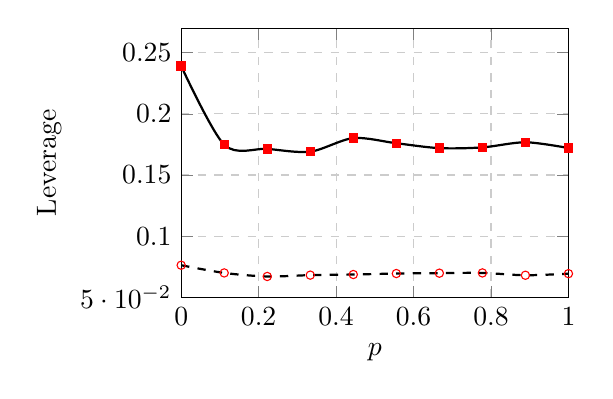
\begin{tikzpicture}
          \begin{axis}[
            ylabel={Leverage},
            ymin=0.05, ymax=0.27,
          ]
            \addplot[only marks, mark=square*, red] coordinates {
              (0.00001,0.2391)            (0.11112,0.1748)            (0.22223,0.1714)            (0.33334,0.1691)            (0.44445,0.1802)            (0.55556,0.1760)            (0.66667,0.1720)            (0.77778,0.1726)            (0.88889,0.1768)            (1.00000,0.1721)
            };
            \addplot[black line] coordinates {
              (0.00001,0.2391)            (0.11112,0.1748)            (0.22223,0.1714)            (0.33334,0.1691)            (0.44445,0.1802)            (0.55556,0.1760)            (0.66667,0.1720)            (0.77778,0.1726)            (0.88889,0.1768)            (1.00000,0.1721)
            };
            \addplot[only marks, mark=o, red] coordinates {
              (0.00001,0.0763)            (0.11112,0.0700)            (0.22223,0.0671)            (0.33334,0.0682)            (0.44445,0.0687)            (0.55556,0.0695)            (0.66667,0.0698)            (0.77778,0.0700)            (0.88889,0.0681)            (1.00000,0.0694)
            };
            \addplot[black line, dashed] coordinates {
              (0.00001,0.0763)            (0.11112,0.0700)            (0.22223,0.0671)            (0.33334,0.0682)            (0.44445,0.0687)            (0.55556,0.0695)            (0.66667,0.0698)            (0.77778,0.0700)            (0.88889,0.0681)            (1.00000,0.0694)
            };
          \end{axis}
        \end{tikzpicture}
      \end{figure}
    \end{column}
    \begin{column}{0.42\textwidth}
      \tiny\renewcommand{\arraystretch}{0.85}\setlength{\tabcolsep}{2pt}
      \begin{tabular}{lrr}
        \toprule
        $p$ & haircut & supply \\
        \midrule
        0.00001 & 0.2391 & 0.0763 \\
        0.111 & 0.1748 & 0.0700 \\
        0.222 & 0.1714 & 0.0671 \\
        0.333 & 0.1691 & 0.0682 \\
        0.444 & 0.1802 & 0.0687 \\
        \textbf{0.556} & \textbf{0.1760} & \textbf{0.0695} \\
        0.667 & 0.1720 & 0.0698 \\
        0.778 & 0.1726 & 0.0700 \\
        0.889 & 0.1768 & 0.0681 \\
        1.000 & 0.1721 & 0.0694 \\
        \bottomrule
      \end{tabular}
    \end{column}
  \end{columns}
\end{frame}

\begin{frame}{Liquidity: haircut ($\blacksquare$) vs.\ supply ($\circ$)}
  \begin{columns}[T]
    \begin{column}{0.55\textwidth}
      \begin{figure}
        \centering
        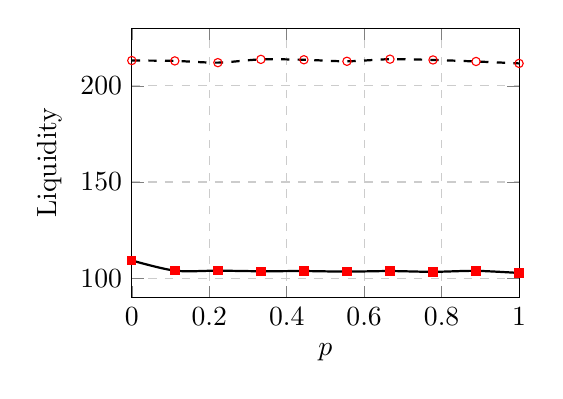
\begin{tikzpicture}
          \begin{axis}[
            ylabel={Liquidity},
            ymin=90, ymax=230,
            scaled y ticks=false,
          ]
            \addplot[only marks, mark=square*, red] coordinates {
              (0.00001,109.2)            (0.11112,103.9)            (0.22223,103.9)            (0.33334,103.6)            (0.44445,103.7)            (0.55556,103.4)            (0.66667,103.7)            (0.77778,103.3)            (0.88889,103.8)            (1.00000,102.7)
            };
            \addplot[black line] coordinates {
              (0.00001,109.2)            (0.11112,103.9)            (0.22223,103.9)            (0.33334,103.6)            (0.44445,103.7)            (0.55556,103.4)            (0.66667,103.7)            (0.77778,103.3)            (0.88889,103.8)            (1.00000,102.7)
            };
            \addplot[only marks, mark=o, red] coordinates {
              (0.00001,213.2)            (0.11112,213.0)            (0.22223,212.1)            (0.33334,213.8)            (0.44445,213.6)            (0.55556,212.8)            (0.66667,213.9)            (0.77778,213.5)            (0.88889,212.7)            (1.00000,211.7)
            };
            \addplot[black line, dashed] coordinates {
              (0.00001,213.2)            (0.11112,213.0)            (0.22223,212.1)            (0.33334,213.8)            (0.44445,213.6)            (0.55556,212.8)            (0.66667,213.9)            (0.77778,213.5)            (0.88889,212.7)            (1.00000,211.7)
            };
          \end{axis}
        \end{tikzpicture}
      \end{figure}
    \end{column}
    \begin{column}{0.42\textwidth}
      \tiny\renewcommand{\arraystretch}{0.85}\setlength{\tabcolsep}{2pt}
      \begin{tabular}{lrr}
        \toprule
        $p$ & haircut & supply \\
        \midrule
        0.00001 & 109.2 & 213.2 \\
        0.111 & 103.9 & 213.0 \\
        0.222 & 103.9 & 212.1 \\
        0.333 & 103.6 & 213.8 \\
        0.444 & 103.7 & 213.6 \\
        \textbf{0.556} & \textbf{103.4} & \textbf{212.8} \\
        0.667 & 103.7 & 213.9 \\
        0.778 & 103.3 & 213.5 \\
        0.889 & 103.8 & 212.7 \\
        1.000 & 102.7 & 211.7 \\
        \bottomrule
      \end{tabular}
    \end{column}
  \end{columns}
\end{frame}

\begin{frame}{Deposits: haircut ($\blacksquare$) vs.\ supply ($\circ$)}
  \begin{columns}[T]
    \begin{column}{0.55\textwidth}
      \begin{figure}
        \centering
        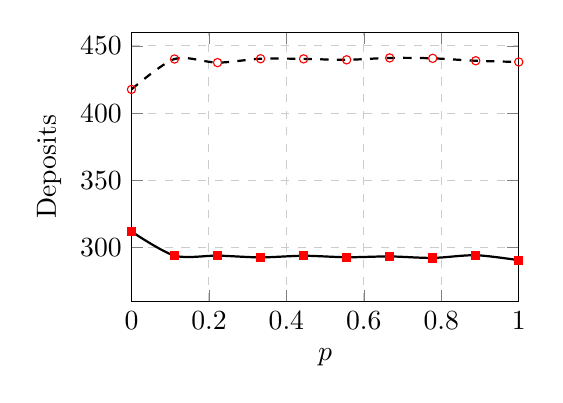
\begin{tikzpicture}
          \begin{axis}[
            ylabel={Deposits},
            ymin=260, ymax=460,
            scaled y ticks=false,
          ]
            \addplot[only marks, mark=square*, red] coordinates {
              (0.00001,312.0)            (0.11112,294.1)            (0.22223,294.1)            (0.33334,292.8)            (0.44445,294.0)            (0.55556,292.9)            (0.66667,293.5)            (0.77778,292.4)            (0.88889,294.4)            (1.00000,290.7)
            };
            \addplot[black line] coordinates {
              (0.00001,312.0)            (0.11112,294.1)            (0.22223,294.1)            (0.33334,292.8)            (0.44445,294.0)            (0.55556,292.9)            (0.66667,293.5)            (0.77778,292.4)            (0.88889,294.4)            (1.00000,290.7)
            };
            \addplot[only marks, mark=o, red] coordinates {
              (0.00001,417.6)            (0.11112,440.2)            (0.22223,437.5)            (0.33334,440.4)            (0.44445,440.3)            (0.55556,439.6)            (0.66667,441.0)            (0.77778,440.7)            (0.88889,438.9)            (1.00000,438.0)
            };
            \addplot[black line, dashed] coordinates {
              (0.00001,417.6)            (0.11112,440.2)            (0.22223,437.5)            (0.33334,440.4)            (0.44445,440.3)            (0.55556,439.6)            (0.66667,441.0)            (0.77778,440.7)            (0.88889,438.9)            (1.00000,438.0)
            };
          \end{axis}
        \end{tikzpicture}
      \end{figure}
    \end{column}
    \begin{column}{0.42\textwidth}
      \tiny\renewcommand{\arraystretch}{0.85}\setlength{\tabcolsep}{2pt}
      \begin{tabular}{lrr}
        \toprule
        $p$ & haircut & supply \\
        \midrule
        0.00001 & 312.0 & 417.6 \\
        0.111 & 294.1 & 440.2 \\
        0.222 & 294.1 & 437.5 \\
        0.333 & 292.8 & 440.4 \\
        0.444 & 294.0 & 440.3 \\
        \textbf{0.556} & \textbf{292.9} & \textbf{439.6} \\
        0.667 & 293.5 & 441.0 \\
        0.778 & 292.4 & 440.7 \\
        0.889 & 294.4 & 438.9 \\
        1.000 & 290.7 & 438.0 \\
        \bottomrule
      \end{tabular}
    \end{column}
  \end{columns}
\end{frame}

\begin{frame}{Equity Lenders: haircut ($\blacksquare$) vs.\ supply ($\circ$)}
  \begin{columns}[T]
    \begin{column}{0.55\textwidth}
      \begin{figure}
        \centering
        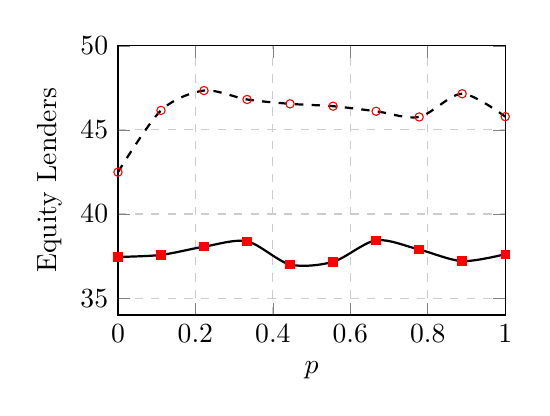
\begin{tikzpicture}
          \begin{axis}[
            ylabel={Equity Lenders},
            ymin=34, ymax=50,
          ]
            \addplot[only marks, mark=square*, red] coordinates {
              (0.00001,37.45)            (0.11112,37.57)            (0.22223,38.06)            (0.33334,38.38)            (0.44445,37.00)            (0.55556,37.16)            (0.66667,38.44)            (0.77778,37.89)            (0.88889,37.20)            (1.00000,37.61)
            };
            \addplot[black line] coordinates {
              (0.00001,37.45)            (0.11112,37.57)            (0.22223,38.06)            (0.33334,38.38)            (0.44445,37.00)            (0.55556,37.16)            (0.66667,38.44)            (0.77778,37.89)            (0.88889,37.20)            (1.00000,37.61)
            };
            \addplot[only marks, mark=o, red] coordinates {
              (0.00001,42.49)            (0.11112,46.16)            (0.22223,47.34)            (0.33334,46.81)            (0.44445,46.55)            (0.55556,46.41)            (0.66667,46.11)            (0.77778,45.77)            (0.88889,47.15)            (1.00000,45.79)
            };
            \addplot[black line, dashed] coordinates {
              (0.00001,42.49)            (0.11112,46.16)            (0.22223,47.34)            (0.33334,46.81)            (0.44445,46.55)            (0.55556,46.41)            (0.66667,46.11)            (0.77778,45.77)            (0.88889,47.15)            (1.00000,45.79)
            };
          \end{axis}
        \end{tikzpicture}
      \end{figure}
    \end{column}
    \begin{column}{0.42\textwidth}
      \tiny\renewcommand{\arraystretch}{0.85}\setlength{\tabcolsep}{2pt}
      \begin{tabular}{lrr}
        \toprule
        $p$ & haircut & supply \\
        \midrule
        0.00001 & 37.45 & 42.49 \\
        0.111 & 37.57 & 46.16 \\
        0.222 & 38.06 & 47.34 \\
        0.333 & 38.38 & 46.81 \\
        0.444 & 37.00 & 46.55 \\
        \textbf{0.556} & \textbf{37.16} & \textbf{46.41} \\
        0.667 & 38.44 & 46.11 \\
        0.778 & 37.89 & 45.77 \\
        0.889 & 37.20 & 47.15 \\
        1.000 & 37.61 & 45.79 \\
        \bottomrule
      \end{tabular}
    \end{column}
  \end{columns}
\end{frame}

\begin{frame}{Equity Borrowers: haircut ($\blacksquare$) vs.\ supply ($\circ$)}
  \begin{columns}[T]
    \begin{column}{0.55\textwidth}
      \begin{figure}
        \centering
        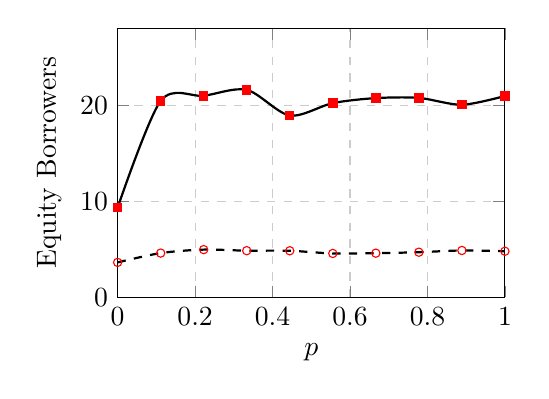
\begin{tikzpicture}
          \begin{axis}[
            ylabel={Equity Borrowers},
            ymin=0, ymax=28,
          ]
            \addplot[only marks, mark=square*, red] coordinates {
              (0.00001,9.34)            (0.11112,20.44)            (0.22223,20.97)            (0.33334,21.59)            (0.44445,18.92)            (0.55556,20.21)            (0.66667,20.73)            (0.77778,20.75)            (0.88889,20.04)            (1.00000,20.95)
            };
            \addplot[black line] coordinates {
              (0.00001,9.34)            (0.11112,20.44)            (0.22223,20.97)            (0.33334,21.59)            (0.44445,18.92)            (0.55556,20.21)            (0.66667,20.73)            (0.77778,20.75)            (0.88889,20.04)            (1.00000,20.95)
            };
            \addplot[only marks, mark=o, red] coordinates {
              (0.00001,3.64)            (0.11112,4.61)            (0.22223,4.97)            (0.33334,4.86)            (0.44445,4.85)            (0.55556,4.57)            (0.66667,4.60)            (0.77778,4.70)            (0.88889,4.88)            (1.00000,4.80)
            };
            \addplot[black line, dashed] coordinates {
              (0.00001,3.64)            (0.11112,4.61)            (0.22223,4.97)            (0.33334,4.86)            (0.44445,4.85)            (0.55556,4.57)            (0.66667,4.60)            (0.77778,4.70)            (0.88889,4.88)            (1.00000,4.80)
            };
          \end{axis}
        \end{tikzpicture}
      \end{figure}
    \end{column}
    \begin{column}{0.42\textwidth}
      \tiny\renewcommand{\arraystretch}{0.85}\setlength{\tabcolsep}{2pt}
      \begin{tabular}{lrr}
        \toprule
        $p$ & haircut & supply \\
        \midrule
        0.00001 & 9.34 & 3.64 \\
        0.111 & 20.44 & 4.61 \\
        0.222 & 20.97 & 4.97 \\
        0.333 & 21.59 & 4.86 \\
        0.444 & 18.92 & 4.85 \\
        \textbf{0.556} & \textbf{20.21} & \textbf{4.57} \\
        0.667 & 20.73 & 4.60 \\
        0.778 & 20.75 & 4.70 \\
        0.889 & 20.04 & 4.88 \\
        1.000 & 20.95 & 4.80 \\
        \bottomrule
      \end{tabular}
    \end{column}
  \end{columns}
\end{frame}

\begin{frame}{Market Power ($\psi$): haircut ($\blacksquare$) vs.\ supply ($\circ$)}
  \begin{columns}[T]
    \begin{column}{0.55\textwidth}
      \begin{figure}
        \centering
        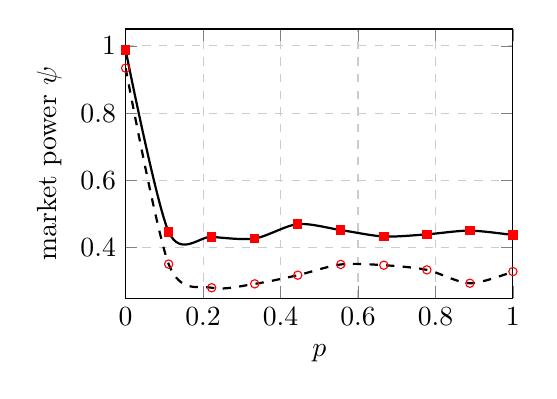
\begin{tikzpicture}
          \begin{axis}[
            ylabel={market power $\psi$},
            ymin=0.25, ymax=1.05,
          ]
            \addplot[only marks, mark=square*, red] coordinates {
              (0.00001,0.9871)            (0.11112,0.4471)            (0.22223,0.4322)            (0.33334,0.4274)            (0.44445,0.4701)            (0.55556,0.4524)            (0.66667,0.4333)            (0.77778,0.4397)            (0.88889,0.4508)            (1.00000,0.4376)
            };
            \addplot[black line] coordinates {
              (0.00001,0.9871)            (0.11112,0.4471)            (0.22223,0.4322)            (0.33334,0.4274)            (0.44445,0.4701)            (0.55556,0.4524)            (0.66667,0.4333)            (0.77778,0.4397)            (0.88889,0.4508)            (1.00000,0.4376)
            };
            \addplot[only marks, mark=o, red] coordinates {
              (0.00001,0.9337)            (0.11112,0.3512)            (0.22223,0.2810)            (0.33334,0.2925)            (0.44445,0.3183)            (0.55556,0.3502)            (0.66667,0.3480)            (0.77778,0.3341)            (0.88889,0.2943)            (1.00000,0.3290)
            };
            \addplot[black line, dashed] coordinates {
              (0.00001,0.9337)            (0.11112,0.3512)            (0.22223,0.2810)            (0.33334,0.2925)            (0.44445,0.3183)            (0.55556,0.3502)            (0.66667,0.3480)            (0.77778,0.3341)            (0.88889,0.2943)            (1.00000,0.3290)
            };
          \end{axis}
        \end{tikzpicture}
      \end{figure}
    \end{column}
    \begin{column}{0.42\textwidth}
      \tiny\renewcommand{\arraystretch}{0.85}\setlength{\tabcolsep}{2pt}
      \begin{tabular}{lrr}
        \toprule
        $p$ & haircut & supply \\
        \midrule
        0.00001 & 0.9871 & 0.9337 \\
        0.111 & 0.4471 & 0.3512 \\
        0.222 & 0.4322 & 0.2810 \\
        0.333 & 0.4274 & 0.2925 \\
        0.444 & 0.4701 & 0.3183 \\
        \textbf{0.556} & \textbf{0.4524} & \textbf{0.3502} \\
        0.667 & 0.4333 & 0.3480 \\
        0.778 & 0.4397 & 0.3341 \\
        0.889 & 0.4508 & 0.2943 \\
        1.000 & 0.4376 & 0.3290 \\
        \bottomrule
      \end{tabular}
    \end{column}
  \end{columns}
\end{frame}

\begin{frame}{Interest Rate ($ir$): haircut ($\blacksquare$) vs.\ supply ($\circ$)}
  \begin{columns}[T]
    \begin{column}{0.55\textwidth}
      \begin{figure}
        \centering
        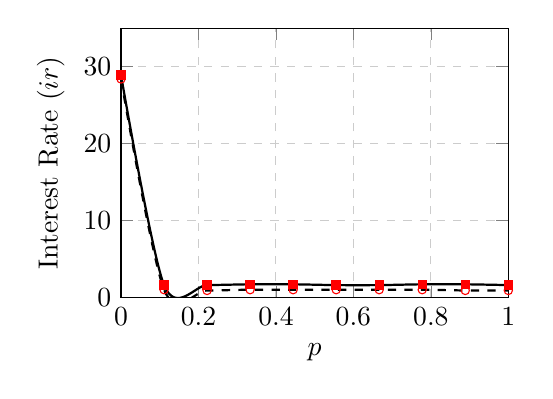
\begin{tikzpicture}
          \begin{axis}[
            ylabel={Interest Rate ($ir$)},
            ymin=0, ymax=35,
          ]
            \addplot[only marks, mark=square*, red] coordinates {
              (0.00001,28.9)            (0.11112,1.6)            (0.22223,1.6)            (0.33334,1.7)            (0.44445,1.7)            (0.55556,1.6)            (0.66667,1.6)            (0.77778,1.7)            (0.88889,1.7)            (1.00000,1.6)
            };
            \addplot[black line] coordinates {
              (0.00001,28.9)            (0.11112,1.6)            (0.22223,1.6)            (0.33334,1.7)            (0.44445,1.7)            (0.55556,1.6)            (0.66667,1.6)            (0.77778,1.7)            (0.88889,1.7)            (1.00000,1.6)
            };
            \addplot[only marks, mark=o, red] coordinates {
              (0.00001,28.4)            (0.11112,1.0)            (0.22223,0.9)            (0.33334,1.0)            (0.44445,1.0)            (0.55556,1.0)            (0.66667,1.0)            (0.77778,1.0)            (0.88889,0.9)            (1.00000,0.9)
            };
            \addplot[black line, dashed] coordinates {
              (0.00001,28.4)            (0.11112,1.0)            (0.22223,0.9)            (0.33334,1.0)            (0.44445,1.0)            (0.55556,1.0)            (0.66667,1.0)            (0.77778,1.0)            (0.88889,0.9)            (1.00000,0.9)
            };
          \end{axis}
        \end{tikzpicture}
      \end{figure}
    \end{column}
    \begin{column}{0.42\textwidth}
      \tiny\renewcommand{\arraystretch}{0.85}\setlength{\tabcolsep}{2pt}
      \begin{tabular}{lrr}
        \toprule
        $p$ & haircut & supply \\
        \midrule
        0.00001 & 28.9 & 28.4 \\
        0.111 & 1.6 & 1.0 \\
        0.222 & 1.6 & 0.9 \\
        0.333 & 1.7 & 1.0 \\
        0.444 & 1.7 & 1.0 \\
        \textbf{0.556} & \textbf{1.6} & \textbf{1.0} \\
        0.667 & 1.6 & 1.0 \\
        0.778 & 1.7 & 1.0 \\
        0.889 & 1.7 & 0.9 \\
        1.000 & 1.6 & 0.9 \\
        \bottomrule
      \end{tabular}
    \end{column}
  \end{columns}
\end{frame}

\begin{frame}{Bad Debt: haircut ($\blacksquare$) vs.\ supply ($\circ$)}
  \begin{columns}[T]
    \begin{column}{0.55\textwidth}
      \begin{figure}
        \centering
        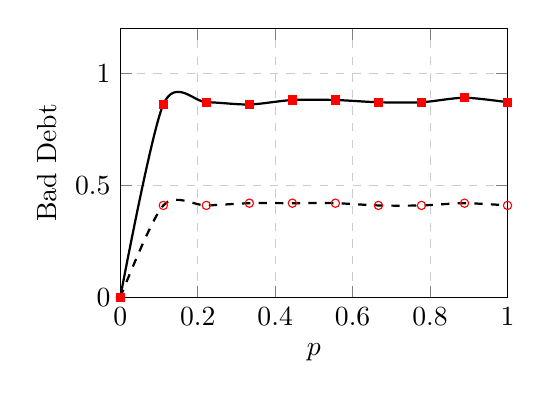
\begin{tikzpicture}
          \begin{axis}[
            ylabel={Bad Debt},
            ymin=0, ymax=1.2,
          ]
            \addplot[only marks, mark=square*, red] coordinates {
              (0.00001,0.00)            (0.11112,0.86)            (0.22223,0.87)            (0.33334,0.86)            (0.44445,0.88)            (0.55556,0.88)            (0.66667,0.87)            (0.77778,0.87)            (0.88889,0.89)            (1.00000,0.87)
            };
            \addplot[black line] coordinates {
              (0.00001,0.00)            (0.11112,0.86)            (0.22223,0.87)            (0.33334,0.86)            (0.44445,0.88)            (0.55556,0.88)            (0.66667,0.87)            (0.77778,0.87)            (0.88889,0.89)            (1.00000,0.87)
            };
            \addplot[only marks, mark=o, red] coordinates {
              (0.00001,0.00)            (0.11112,0.41)            (0.22223,0.41)            (0.33334,0.42)            (0.44445,0.42)            (0.55556,0.42)            (0.66667,0.41)            (0.77778,0.41)            (0.88889,0.42)            (1.00000,0.41)
            };
            \addplot[black line, dashed] coordinates {
              (0.00001,0.00)            (0.11112,0.41)            (0.22223,0.41)            (0.33334,0.42)            (0.44445,0.42)            (0.55556,0.42)            (0.66667,0.41)            (0.77778,0.41)            (0.88889,0.42)            (1.00000,0.41)
            };
          \end{axis}
        \end{tikzpicture}
      \end{figure}
    \end{column}
    \begin{column}{0.42\textwidth}
      \tiny\renewcommand{\arraystretch}{0.85}\setlength{\tabcolsep}{2pt}
      \begin{tabular}{lrr}
        \toprule
        $p$ & haircut & supply \\
        \midrule
        0.00001 & 0.00 & 0.00 \\
        0.111 & 0.86 & 0.41 \\
        0.222 & 0.87 & 0.41 \\
        0.333 & 0.86 & 0.42 \\
        0.444 & 0.88 & 0.42 \\
        \textbf{0.556} & \textbf{0.88} & \textbf{0.42} \\
        0.667 & 0.87 & 0.41 \\
        0.778 & 0.87 & 0.41 \\
        0.889 & 0.89 & 0.42 \\
        1.000 & 0.87 & 0.41 \\
        \bottomrule
      \end{tabular}
    \end{column}
  \end{columns}
\end{frame}

\begin{frame}{Loans: haircut ($\blacksquare$) vs.\ supply ($\circ$)}
  \begin{columns}[T]
    \begin{column}{0.55\textwidth}
      \begin{figure}
        \centering
        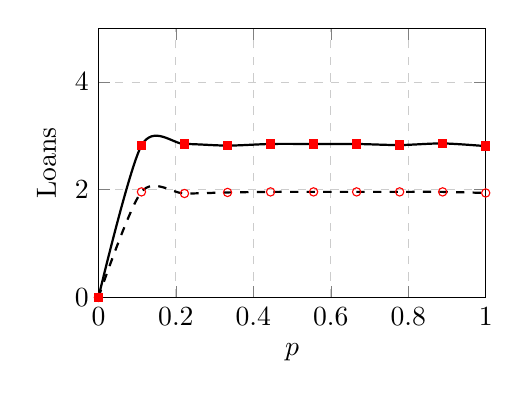
\begin{tikzpicture}
          \begin{axis}[
            ylabel={Loans},
            ymin=0, ymax=5,
          ]
            \addplot[only marks, mark=square*, red] coordinates {
              (0.00001,0.00)            (0.11112,2.82)            (0.22223,2.85)            (0.33334,2.82)            (0.44445,2.85)            (0.55556,2.85)            (0.66667,2.85)            (0.77778,2.83)            (0.88889,2.86)            (1.00000,2.81)
            };
            \addplot[black line] coordinates {
              (0.00001,0.00)            (0.11112,2.82)            (0.22223,2.85)            (0.33334,2.82)            (0.44445,2.85)            (0.55556,2.85)            (0.66667,2.85)            (0.77778,2.83)            (0.88889,2.86)            (1.00000,2.81)
            };
            \addplot[only marks, mark=o, red] coordinates {
              (0.00001,0.00)            (0.11112,1.96)            (0.22223,1.93)            (0.33334,1.95)            (0.44445,1.96)            (0.55556,1.96)            (0.66667,1.96)            (0.77778,1.96)            (0.88889,1.96)            (1.00000,1.94)
            };
            \addplot[black line, dashed] coordinates {
              (0.00001,0.00)            (0.11112,1.96)            (0.22223,1.93)            (0.33334,1.95)            (0.44445,1.96)            (0.55556,1.96)            (0.66667,1.96)            (0.77778,1.96)            (0.88889,1.96)            (1.00000,1.94)
            };
          \end{axis}
        \end{tikzpicture}
      \end{figure}
    \end{column}
    \begin{column}{0.42\textwidth}
      \tiny\renewcommand{\arraystretch}{0.85}\setlength{\tabcolsep}{2pt}
      \begin{tabular}{lrr}
        \toprule
        $p$ & haircut & supply \\
        \midrule
        0.00001 & 0.00 & 0.00 \\
        0.111 & 2.82 & 1.96 \\
        0.222 & 2.85 & 1.93 \\
        0.333 & 2.82 & 1.95 \\
        0.444 & 2.85 & 1.96 \\
        \textbf{0.556} & \textbf{2.85} & \textbf{1.96} \\
        0.667 & 2.85 & 1.96 \\
        0.778 & 2.83 & 1.96 \\
        0.889 & 2.86 & 1.96 \\
        1.000 & 2.81 & 1.94 \\
        \bottomrule
      \end{tabular}
    \end{column}
  \end{columns}
\end{frame}

\begin{frame}{Prob. of Bankruptcy ($p_b$): haircut ($\blacksquare$) vs.\ supply ($\circ$)}
  \begin{columns}[T]
    \begin{column}{0.55\textwidth}
      \begin{figure}
        \centering
        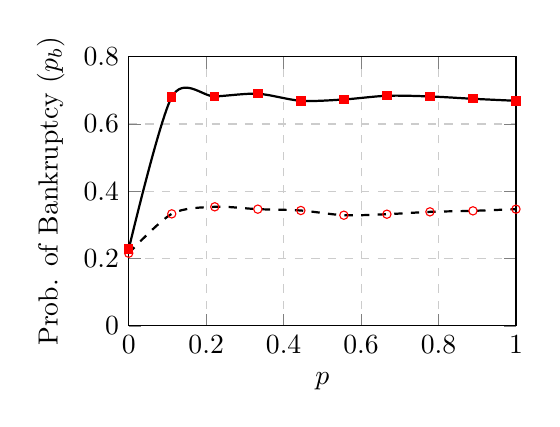
\begin{tikzpicture}
          \begin{axis}[
            ylabel={Prob. of Bankruptcy ($p_b$)},
            ymin=0, ymax=0.8,
          ]
            \addplot[only marks, mark=square*, red] coordinates {
              (0.00001,0.228)            (0.11112,0.680)            (0.22223,0.682)            (0.33334,0.690)            (0.44445,0.669)            (0.55556,0.673)            (0.66667,0.684)            (0.77778,0.682)            (0.88889,0.675)            (1.00000,0.669)
            };
            \addplot[black line] coordinates {
              (0.00001,0.228)            (0.11112,0.680)            (0.22223,0.682)            (0.33334,0.690)            (0.44445,0.669)            (0.55556,0.673)            (0.66667,0.684)            (0.77778,0.682)            (0.88889,0.675)            (1.00000,0.669)
            };
            \addplot[only marks, mark=o, red] coordinates {
              (0.00001,0.216)            (0.11112,0.333)            (0.22223,0.354)            (0.33334,0.347)            (0.44445,0.343)            (0.55556,0.329)            (0.66667,0.332)            (0.77778,0.339)            (0.88889,0.342)            (1.00000,0.347)
            };
            \addplot[black line, dashed] coordinates {
              (0.00001,0.216)            (0.11112,0.333)            (0.22223,0.354)            (0.33334,0.347)            (0.44445,0.343)            (0.55556,0.329)            (0.66667,0.332)            (0.77778,0.339)            (0.88889,0.342)            (1.00000,0.347)
            };
          \end{axis}
        \end{tikzpicture}
      \end{figure}
    \end{column}
    \begin{column}{0.42\textwidth}
      \tiny\renewcommand{\arraystretch}{0.85}\setlength{\tabcolsep}{2pt}
      \begin{tabular}{lrr}
        \toprule
        $p$ & haircut & supply \\
        \midrule
        0.00001 & 0.228 & 0.216 \\
        0.111 & 0.680 & 0.333 \\
        0.222 & 0.682 & 0.354 \\
        0.333 & 0.690 & 0.347 \\
        0.444 & 0.669 & 0.343 \\
        \textbf{0.556} & \textbf{0.673} & \textbf{0.329} \\
        0.667 & 0.684 & 0.332 \\
        0.778 & 0.682 & 0.339 \\
        0.889 & 0.675 & 0.342 \\
        1.000 & 0.669 & 0.347 \\
        \bottomrule
      \end{tabular}
    \end{column}
  \end{columns}
\end{frame}

\end{document}